\section{Theorie}
\label{sec:Theorie}

Seit einigen Jahren findet Mikrowellen-Strahlung in vielen Bereichen eine Anwendung. 
Den meisten Leuten fällt beim Begriff Mikrowelle vermutlich als erstes der Mirkowellen-Ofen ein,
da dieses Gerät ein wichtiger Bestandteil vieler Küchen heutzutage ist.
Aber Mikrowellen haben noch deutlich mehr Anwendungsgebiete:
\begin{itemize}
    \item jegliche Art der kabellosen Kommunikation. (Mobilfunk, WLAN, Bluetooth,...)
    \item Radartechnik
    \item Navigation über GPS
    \item Radioastronomie
    \item Spektroskopie
    \item ...
\end{itemize}

Das Wort \enquote{Mikrowellen} ist allerdings irreführend, da die Wellenlänge von elektromagnetischer Strahlung in der Größenordnung Mikrometer 
Infrarot-Strahlung ist.
Mikrowellen-Strahlung liegt hingegen im Wellenlängenbereich von Millimeter bis Meter bzw. einem Frequenzbereich von $\SI{300}{\mega\hertz}$ bis $\SI{300}{\giga\hertz}$.
Und das \enquote{Mikro} in Mikrowellen steht eher für klein als für die Größenordnung.

Für die nahezu dispersionsfreie Übertragung von Mikrowellen werden Hohlleiter verwendet.

\subsection{Erzeugung von Mikrowellen mittels eines Reflexklystrons}
\label{ssec:Erzeugung}

Um Mikrowellen-Strahlung mit einer hohen Intensität erzeugen zu können, hat man ein sogenanntes Klystron entwickelt.
Da diese Klystrons allerdings groß sind, wurden sie zum sogenannten Reflexklystron weiterentwickelt.
Die Funktionsweise des Reflexklystrons ist sehr ähnlich zum Klystron und lässt sich besser am Klystron erklären.
Beide Geräte sind in \autoref{fig:wiki_klystron} schematisch dargestellt.

\begin{figure}
    \centering
    \begin{subfigure}{0.45\textwidth}
        \centering
        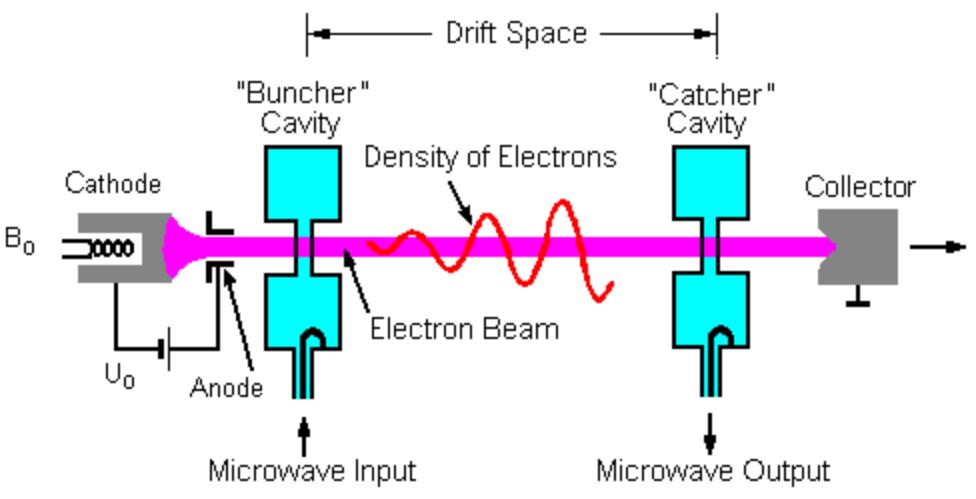
\includegraphics[width=\textwidth]{images/klystron.png}
        \caption{Klystron}
        \label{fig:klystron}
    \end{subfigure}
    \begin{subfigure}{0.45\textwidth}
        \centering
        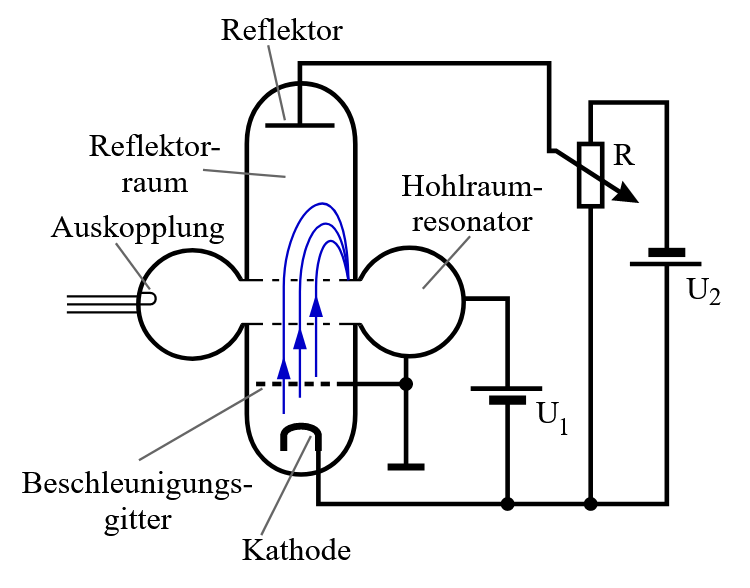
\includegraphics[width=\textwidth]{images/reflexklystron.png}
        \caption{Reflexklystron}
        \label{fig:reflexklystron}
    \end{subfigure}
    \caption{Schematische Skizzen vom Klystron und Reflexklystron \cite{wiki_klystron}}
    \label{fig:wiki_klystron}
\end{figure}

Elektronen werden von einer Glühkathode aus beschleunigt. 
Diese treten dann in einen \enquote{Buncher} Hohlraum ein.
In diesem Hohlraum schwingt ein elektrisches, annähernd homogenes Feld parallel zur Bewegungsrichtung der Elektronen.
Diese Schwingung wird durch ein Eingangssignal angeregt und der Hohlraum funktioniert auf dem Prinzip eines RC-Schwingkreises,
wobei in der Mitte ein Kondensator und außen eine Art Spule mit einer Windung ist.
Durch das schwingende elektrische Feld werden die Elektronen unterschiedlich stark beschleunigt oder abgebremst (Geschwindigkeitsmodulation)
und es entstehen auf dem Weg zum nächsten Hohlraum \enquote{Bunches}, also Häufungen von Elektronen. (Dichtemodulation)

In dem \enquote{Catcher} Hohlraum sollten die Elektronbunches genau so ankommen, dass sie die Resonanzfrequenz des Hohlraums treffen und dort die Schwingung anregen.
Da allerdings hier die Elektronen sehr stark abgebremst werden, wird viel Energie in die angeregte Schwingung abgegeben 
und das so erzeugte Ausgangssignal hat eine deutlich höher Intensität als das Eingangssignal.

Beim Reflexklystron erfüllt ein Hohlraum beide soeben beschriebenen Funktionen und die Elektronen werden durch einen Reflektor in den gleichen Hohlraum zurückgeleitet.
Die so entstandene Schwingung kann z.B. über einen Draht oder einen Hohlleiter ausgekoppelt werden.

Da die Elektronen zum richtigen Zeitpunkt und in Bunches auf dem Rückweg wieder im Hohlraum ankommen müssen, 
müssen die Beschleunigungsspannung, die Reflektorspannung und die Abmessungen des Hohlraums
so angepasst werden, dass eine maximale Ausgangsleistung erreicht wird.
Eine optimale Flugdauer der Elektronen ist 
\begin{equation}
    \tau = T_0 (N+3/4) \, ,
\end{equation}
wobei $T_0$ die Periodenlänge bei Resonanz des Hohlraums ist und $N$ eine natürliche Zahl (oder 0) ist.
Wie sich Amplitude und Frequenz des Ausgangssignals durch die Reflektorspannung verändert ist in \autoref{fig:modulation} zu sehen.

\begin{figure}
    \centering
    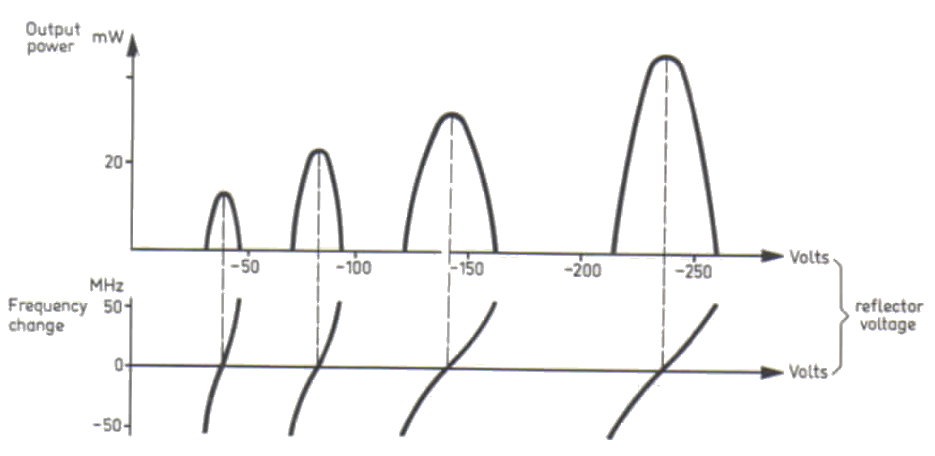
\includegraphics[width=0.7\textwidth]{images/modulation_white.png}
    \caption{Amplituden- und Frequenzmodulation des Reflexklystrons in Abhängigkeit der Reflektorspannung \cite{V53_old}}
    \label{fig:modulation}
\end{figure}

\subsection{Mikrowellen auf Hohlleitern}
\label{ssec:Hohlleiter}

Eine Möglichkeit Wellen über eine große Strecke mit nahezu keiner Dispersion zu übertragen sind Hohlleiter.
Im Fall von elektromagnetischer Strahlung werden als Hohlleiter Metallrohre verwendet, die meistens Luft enthalten und einen rechteckigen Querschnitt haben.
Dadurch, dass die Welle an den Wänden reflektiert wird entsteht in der $xy$-Ebene eine stehende Welle, wenn die $z$-Richtung die Ausbreitungsrichtung ist.

Wir beschränken uns hier auf die Betrachtung von rechteckigen Hohlleitern mit den Kantenlängen $a$ ($x$-Achse) und $b$ ($y$-Achse).
Außerdem definieren wir o.B.d.A $a \geq b$.
Die Wellen im Hohlleiter können verschiedene Formen annehmen. 
Diese Form wird als Modus bezeichnet und durch die Zahlen $m,n \in \mathbb{N}_0$ gekennzeichnet, je nachdem wie viele Wellenbäuche in die $x$- oder $y$-Richtung liegen.
Außerdem können entweder das elektrische, das magnetische oder beide Felder senkrecht zur Ausbreitungsrichtung stehen.
Ein Modus wird so eindeutig über $\symup{TE}_{m,n}$, $\symup{TM}_{m,n}$ oder $\symup{TEM}_{m,n}$ gekennzeichnet. 
Ein Beispiel-Modus ist in \autoref{fig:hohlleiter_TE10} zu sehen.

\begin{figure}
    \centering
    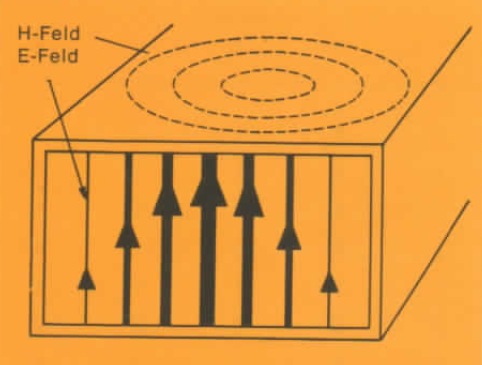
\includegraphics[width=0.4\textwidth]{images/hohlleiter_TE10.png}
    \caption{Skizze einer $\symup{TE}_{1,0}$ Mode in einem rechteckigen Hohlleiter \cite{V53_old}}
    \label{fig:hohlleiter_TE10}
\end{figure}

Schickt man nun eine elektromagnetische Welle mit der Wellenlänge $\lambda_0$ durch so einen Hohlleiter,
dann vergrößert sich diese Wellenlänge zu
\begin{equation}
    \lambda_\text{H} = \frac{\lambda_0}{ \sqrt{ 1 - \left( \frac{\lambda_0}{\lambda_\text{G}} \right)^2 } } \, ,
\end{equation}
wobei $\lambda_\text{H}$ die Wellenlänge im Hohlleiter ist und $\lambda_\text{G}$ die kleinstmögliche Wellenlänge bzw. die Grenzwellenlänge im Hohlleiter ist.
Diese Grenzwellenlänge kann über
\begin{equation}
    \lambda_\text{G} = \frac{2}{ \sqrt{ \left( \frac{m}{a} \right)^2 + \left( \frac{n}{b} \right)^2 } }
\end{equation}
für den jeweiligen Hohlleiter berechnet werden.

Meistens wird ein Hohlleiter im niedrigsten Modus verwendet.
Für den $\symup{TE}_{1,0}$-Modus kann nun mit $f=c/\lambda_0$ die Frequenz einer einlaufenden Welle über
\begin{equation}
    f = c \cdot \sqrt{ \left( \lambda_\text{H} \right)^{-2} + \left( 2 \cdot a \right)^{-2} }
    \label{eq:frequenz}
\end{equation}
bestimmt werden.

In einen Hohlleiter kann ein sogenanntes Dämpfungsglied eingebaut werden, das die Leistung der übertragenen Welle abschwächt.
Die Dämpfung wird dabei in $\si{\decibel}$ angegeben.

\subsection{Stehwellenverhältnis und dessen Messmethoden}
\label{ssec:Stehwellenverhältnis}

Eine Übertragungsleitung wie ein Hohlleiter ist immer verlustbehaftet und Störfaktoren können nie vollkommen verhindert werden.
Einer dieser Störfaktoren sind Reflektionen an Unreinheiten der Leitung oder an einem Übergang an eine Last, die eine nicht passende Impedanz hat.
Die Wechselwirkung einer einlaufenden mit einer reflektierten Welle erzeugt dann eine stehende Welle.
Das sogenannte Stehwellenverhältnis $S$ (bzw. SWR für \enquote{standing wave ratio}) ist ein Maß für die Abschwächung der Leistung durch reflektierte Wellen.
Es ist definiert über das Verhältnis der Feldstärken
\begin{equation}
    S = \frac{E_\text{max}}{E_\text{min}}
\end{equation}
und wird auch als Welligkeit bezeichnet.

Eine Größe, die damit in Verbindung steht ist der Spannungs-Reflexionskoeffizient $\rho$.
Dieser ist definiert über das Verhältnis von reflektierter zu einlaufender Feldstärke 
und hängt mit $S$ über
\begin{equation}
    | \rho | = \frac{S-1}{S+1}
\end{equation}
zusammen.

\subsubsection{Direkte Messmethode}
\label{sssec:Direkte_Messmethode}

Um das Stehwellenverhältnis direkt zu messen, wird in die zu vermessende Leitung eine kapazitive Sonde eingeführt, 
die einen Bruchteil des übertragenen Signals auskoppelt und an einen hochsensitiven Spannungsmesser weiterleitet.
Das Stehwellenverhältnis kann dann über
\begin{equation}
    S = \frac{U_\text{max}}{U_\text{min}}
    \label{eq:Direkte_Methode}
\end{equation}
berechnet werden.
In diesem Versuch wird ein SWR-Messer verwendet, der das Stehwellenverhältnis direkt ausgibt.

\subsubsection{\texorpdfstring{$\SI{3}{\decibel}$-Messmethode}{3dB-Messmethode}}
\label{sssec:3dB_Messmethode}

Eine Methode die Spannungsüberlastung des SWR-Messers zu umgehen ist die $\SI{3}{\decibel}$-Methode.
Anstatt das Minimum und das Maximum der Spannung zu messen, 
wird hier nur die doppelte Spannung des Minimums gemessen.
Diese Werte der Spannung müssen allerdings an zwei aufeinander folgenden Stellen gemessen werden 
und mit dem Abstand $\Delta d$ kann dann das Stehwellenverhältnis über
\begin{equation}
    S = \sqrt{1 + \sin^{-2}\left( \frac{\pi \cdot \Delta d}{\lambda_\text{H}} \right)}
    \label{eq:3dB_Methode}
\end{equation}
bestimmt werden.
Diese Gleichung kann zu 
\begin{equation}
    S = \frac{\lambda_\text{H}}{\pi \cdot \Delta d}
    \label{eq:3dB_Methode_genähert}
\end{equation}
genähert werden, wenn $S \gtrsim 10$ ist.

\subsubsection{Abschwächer-Messmethode}
\label{sssec:Abschwächer_Messmethode}

Der verwendete SWR-Detektor zeigt ein quadratisches Verhalten solange die Ausgangsspannung zur Eingangsspannung proportional ist.
Eine Möglichkeit das Stehwellenverhältnis zu messen, wenn dies nicht der Fall ist, ist die Abschwächer-Methode.
Das Signal wird hier durch ein Dämpfungsglied zwischen Generator und Messleitung so abgeschwächt, dass das Maximum gerade so hoch ist wie das Minimum vor der Abschwächung.
Mit der Differenz $\Delta A$ eingestellten Dämpfungen vor und nach der Abschwächung kann dann das Stehwellenverhältnis über
\begin{equation}
    S = 10^{\frac{\Delta A}{20}}
    \label{eq:Abschwächer_Methode}
\end{equation}
berechnet werden.
